\documentclass[12pt]{article}
\usepackage{graphicx}
\usepackage{geometry}
\usepackage{setspace}
\usepackage{titlesec}
\usepackage{tocloft}
\usepackage{fancyhdr}
\usepackage{hyperref}
\usepackage{xcolor}
\usepackage[T1]{fontenc}
\usepackage[utf8]{inputenc}
\usepackage[ngerman]{babel}

\geometry{a4paper, margin=2.5cm}
\setstretch{1.5}
\titleformat{\section}[block]{\LARGE\bfseries\color{black}}{}{0em}{\filcenter}
\titlespacing*{\section}{0pt}{3.5ex plus 1ex minus .2ex}{2.3ex plus .2ex}
\renewcommand{\cftsecleader}{\cftdotfill{\cftdotsep}}
\renewcommand{\contentsname}{Inhaltsverzeichnis}
\renewcommand{\cftaftertoctitle}{\par\nobreak\bigskip\bigskip\bigskip}
\setlength{\cftbeforesecskip}{0.5em}
\setlength{\cftaftertoctitleskip}{2cm}
\hypersetup{
    colorlinks=true,
    linkcolor=blue,
    filecolor=magenta,
    urlcolor=cyan,
}

\pagestyle{fancy}
\fancyhf{}
\fancyhead[R]{\thepage}
\fancyhead[L]{\nouppercase{\leftmark}}
\renewcommand{\headrulewidth}{0pt}
\fancyfoot[C]{\thepage}
\renewcommand{\footrulewidth}{0pt}

\definecolor{lightgray}{RGB}{240,240,240}

\begin{document}

\begin{titlepage}
    \centering
    \vspace*{3cm}
    {\Huge\bfseries\textcolor{blue}{\MakeUppercase{ Claras Chaos-Kontinent }}\par}
    \vspace{0.5cm}
    {\Large\textit{ Maja Schmidt }\par}
    \vfill
    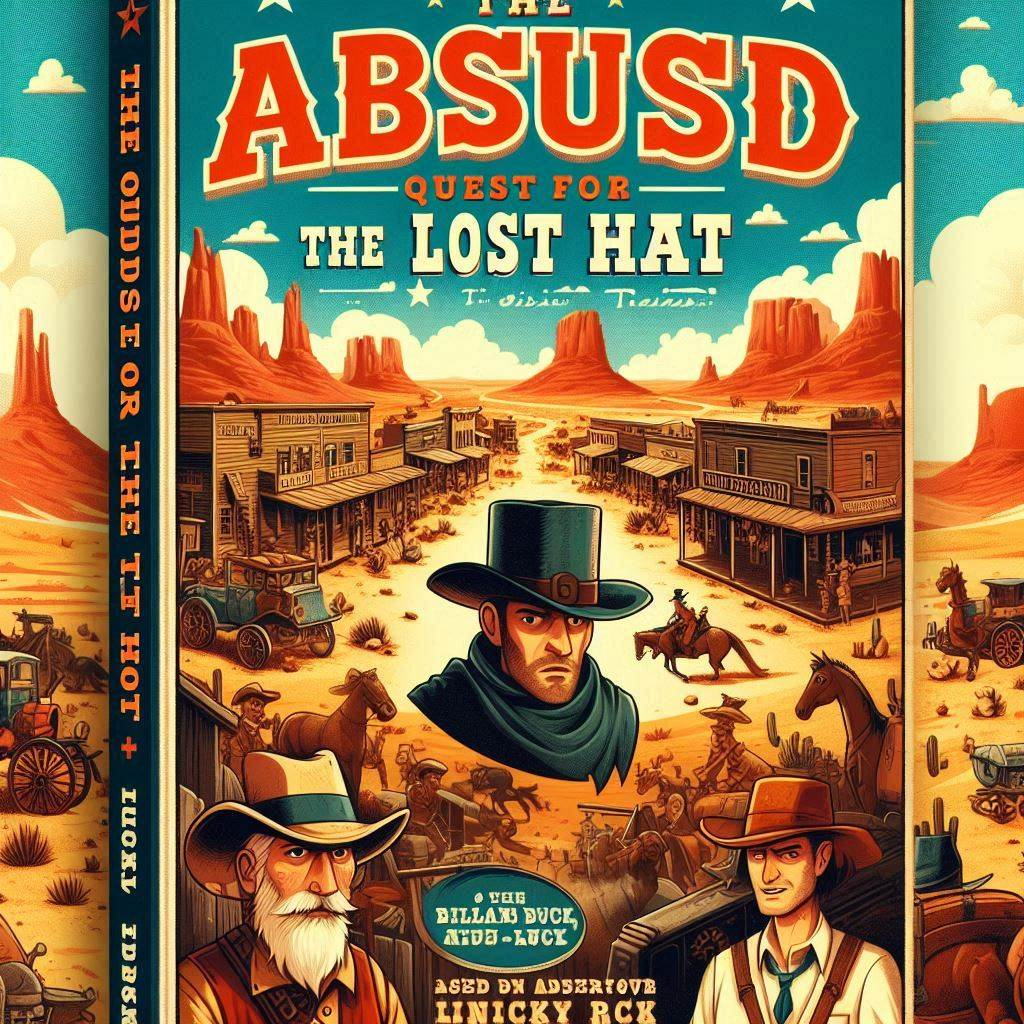
\includegraphics[width=0.9\textwidth]{ cover.jpg }
    \vfill
    \today
\end{titlepage}

\section*{Autorenvita}
\vspace{4cm}
Maja Schmidt ist eine erfahrene und bekannte Autorin von Kinderbüchern, die sich auf Geschichten über mutige Mädchen spezialisiert hat, die die Welt erkunden. Mit ihrem humorvollen und fantasievollen Schreibstil begeistert sie junge Leserinnen und Leser und inspiriert sie, neugierig und abenteuerlustig zu sein. Maja lebt mit ihrer Familie und zwei Katzen in einer kleinen Stadt und liebt es, neue Orte zu entdecken und ihre Erlebnisse in ihren Büchern zu teilen.

\clearpage
\tableofcontents
\clearpage


\section{ Die magische Landkarte }
 Es war ein regnerischer Nachmittag in Waldhausen, und Clara hatte nichts Besseres zu tun, als den Dachboden ihrer Großmutter zu erkunden. Der Dachboden war ein wahres Paradies für ein neugieriges Mädchen wie sie, vollgestopft mit alten Kisten, verstaubten Büchern und geheimnisvollen Gegenständen. Während sie durch die Kisten stöberte, stieß sie auf eine besonders alte und verstaubte Truhe. Mit einem kräftigen Ruck öffnete sie den Deckel und entdeckte darin eine alte, vergilbte Landkarte.

'Was ist das denn?' murmelte Clara und zog die Karte vorsichtig heraus. Sie pustete den Staub weg und betrachtete die seltsamen Symbole und Linien darauf. Plötzlich begann die Karte zu leuchten, und Clara konnte ihren Augen kaum trauen. Die Linien und Symbole formten sich zu einem Bild, das einen geheimen Kontinent zeigte.

'Wow, das ist ja unglaublich!' rief Clara aus. In diesem Moment hörte sie eine leise Stimme hinter sich.

'Du hast die Karte gefunden, Clara. Das ist der erste Schritt zu einem großen Abenteuer.'

Clara drehte sich um und sah einen kleinen, glänzenden Kompass auf dem Boden liegen. Zu ihrer Überraschung sprach der Kompass weiter.

'Ich bin der sprechende Kompass, und ich werde dich auf deinem Abenteuer führen.'

Clara hob den Kompass auf und betrachtete ihn neugierig. 'Ein sprechender Kompass? Das ist ja verrückt!'

Der Kompass lachte. 'Ja, das sagen die meisten. Aber glaub mir, du wirst mich noch brauchen. Der Chaos-Kontinent ist voller Überraschungen und Herausforderungen.'

Clara konnte ihre Aufregung kaum verbergen. 'Dann lass uns keine Zeit verlieren! Wohin gehen wir zuerst?'

Der Kompass drehte sich in Claras Hand und zeigte auf die leuchtende Karte. 'Folge einfach der Karte, und ich werde dir den Weg weisen.'

Mit einem letzten Blick auf den Dachboden ihrer Großmutter machte sich Clara auf den Weg. Sie wusste, dass dies der Beginn eines unglaublichen Abenteuers war, und sie konnte es kaum erwarten, zu sehen, was der Chaos-Kontinent für sie bereithielt. Clara folgte der leuchtenden Karte, die sie durch den Dachboden führte. Plötzlich begann der Raum um sie herum zu verschwimmen, und sie fand sich in einer völlig neuen Welt wieder. Der Boden unter ihren Füßen war weich und federnd, und die Luft roch nach frischen Blumen und Abenteuer.

'Willkommen auf dem Chaos-Kontinent!' rief der sprechende Kompass fröhlich. 'Hier beginnt unser Abenteuer richtig.'

Clara sah sich um und entdeckte eine Gruppe von Bäumen, die sich im Wind wiegten. Doch als sie näher kam, bemerkte sie, dass die Bäume nicht nur im Wind tanzten, sondern tatsächlich tanzten! Die Äste bewegten sich im Takt einer unsichtbaren Melodie, und die Blätter raschelten wie Applaus.

'Das sind die tanzenden Bäume,' erklärte der Kompass. 'Sie sind freundlich, aber sie können auch sehr schelmisch sein.'

Clara lachte und winkte den Bäumen zu. 'Hallo, ihr tanzenden Bäume! Könnt ihr mir den Weg zeigen?'

Die Bäume hielten kurz inne, dann neigten sie sich in eine Richtung und bildeten einen Pfad. Clara folgte dem Pfad, der sie zu einem glitzernden Fluss führte. Das Wasser war nicht klar, sondern schimmerte in allen Farben des Regenbogens.

'Das ist der Limonadenfluss,' sagte der Kompass. 'Er sieht schön aus, aber sei vorsichtig. Er ist sehr klebrig.'

Clara kniete sich hin und tauchte einen Finger ins Wasser. 'Es schmeckt wirklich nach Limonade!' rief sie erstaunt. 'Aber wie sollen wir ihn überqueren?'

In diesem Moment hörte sie ein freches Lachen. Ein bunter Papagei flatterte heran und setzte sich auf einen Ast in ihrer Nähe. 'Wenn du den Fluss überqueren willst, musst du erst mein Rätsel lösen,' sagte der Papagei mit einem schelmischen Grinsen.

Clara nickte entschlossen. 'Okay, was ist dein Rätsel?'

Der Papagei krächzte und sprach: 'Ich bin leicht wie eine Feder, doch kein Vogel. Ich kann fliegen, doch habe keine Flügel. Was bin ich?'

Clara dachte nach. 'Leicht wie eine Feder, kann fliegen, aber kein Vogel... Ein Luftballon!'

Der Papagei lachte und nickte. 'Richtig! Du hast das Rätsel gelöst. Hier ist dein Preis.' Er schnappte sich einen Ast und legte ihn über den Fluss, der sich sofort in eine stabile Brücke verwandelte.

Clara überquerte die Brücke und winkte dem Papagei zu. 'Danke, frecher Papagei!'

Der Papagei zwinkerte ihr zu. 'Vielleicht sehen wir uns wieder, Clara. Viel Glück auf deinem Abenteuer!'

Mit einem Lächeln auf den Lippen und dem sprechenden Kompass in der Hand setzte Clara ihren Weg fort. Sie wusste, dass noch viele Herausforderungen und Überraschungen auf sie warteten, aber sie fühlte sich bereit, ihnen entgegenzutreten. Clara und der sprechende Kompass setzten ihren Weg fort, als sie plötzlich ein leises Summen hörten. Sie folgten dem Geräusch und fanden sich bald in einem Wald wieder, wo die Bäume nicht nur tanzten, sondern auch leise sangen. Die Melodie war beruhigend und Clara fühlte sich, als ob sie in einem Traum wandelte.

'Das ist der Wald der tanzenden Bäume,' sagte der Kompass. 'Hier sind die Bäume nicht nur schelmisch, sondern auch musikalisch.'

Clara lächelte und lauschte der Melodie. 'Es ist wunderschön hier. Aber wie finden wir den Weg weiter?'

Die Bäume schienen ihre Frage zu hören und begannen, sich in eine Richtung zu neigen, als ob sie einen unsichtbaren Pfad bildeten. Clara folgte dem Pfad, der sie tiefer in den Wald führte. Plötzlich hörte sie ein bekanntes Lachen.

'Na, Clara, hast du schon genug von Abenteuern?' fragte der freche Papagei, der auf einem Ast über ihr saß.

Clara lachte. 'Noch lange nicht! Was hast du diesmal für mich?'

Der Papagei flatterte hinunter und setzte sich auf Claras Schulter. 'Ich habe ein weiteres Rätsel für dich. Bist du bereit?'

Clara nickte entschlossen. 'Immer bereit!'

Der Papagei krächzte und sprach: 'Ich habe Städte, aber keine Häuser. Ich habe Berge, aber keine Bäume. Ich habe Wasser, aber keine Fische. Was bin ich?'

Clara dachte nach. 'Städte ohne Häuser, Berge ohne Bäume, Wasser ohne Fische... Eine Landkarte!'

Der Papagei lachte und nickte. 'Richtig! Du bist wirklich schlau, Clara. Hier ist dein nächster Hinweis.' Er schnappte sich ein Blatt und ließ es vor Clara fallen. Auf dem Blatt war eine kleine Zeichnung eines Schlüssels.

'Ein Schlüssel?' fragte Clara verwirrt. 'Wofür ist der?'

Der Papagei zwinkerte. 'Das wirst du bald herausfinden. Viel Glück, Clara!'

Mit dem Blatt in der Hand und einem Lächeln auf den Lippen setzte Clara ihren Weg fort. Der sprechende Kompass führte sie weiter durch den Wald, bis sie schließlich vor einer großen, alten Tür standen, die in einen Baum eingelassen war.

'Das ist es,' sagte der Kompass. 'Der Schlüssel auf dem Blatt wird dir helfen, diese Tür zu öffnen.'

Clara hielt das Blatt vor die Tür, und plötzlich begann die Tür zu leuchten und öffnete sich langsam. Dahinter lag ein wunderschöner Garten, voller bunter Blumen und exotischer Pflanzen.

'Willkommen im Garten der Geheimnisse,' sagte der Kompass. 'Hier wirst du viele Antworten finden.'

Clara trat in den Garten und fühlte sich, als ob sie in eine andere Welt eingetreten wäre. Sie wusste, dass dies erst der Anfang ihres großen Abenteuers war und dass noch viele Herausforderungen und Überraschungen auf sie warteten. Aber mit ihren neuen Freunden an ihrer Seite fühlte sie sich bereit, alles zu meistern.

\section{ Abenteuer auf dem Chaos-Kontinent }
 Clara trat vorsichtig durch die leuchtende Tür und fand sich in einem magischen Garten wieder. Überall blühten bunte Blumen, und exotische Pflanzen wuchsen in allen Formen und Größen. Der sprechende Kompass schwebte neben ihr und zeigte ihr den Weg.

'Das ist unglaublich,' flüsterte Clara, während sie die Schönheit um sich herum bewunderte.

'Warte nur, bis du den Rest des Chaos-Kontinents siehst,' antwortete der Kompass mit einem Augenzwinkern.

Sie folgten einem schmalen Pfad, der sich durch den Garten schlängelte, bis sie schließlich an den Rand des Gartens kamen. Vor ihnen erstreckte sich ein dichter Wald, und die Bäume schienen sich im Takt einer unsichtbaren Melodie zu wiegen.

'Das muss der Wald der tanzenden Bäume sein,' sagte Clara aufgeregt.

'Genau,' bestätigte der Kompass. 'Hier sind die Bäume nicht nur schelmisch, sondern auch musikalisch.'

Clara trat vorsichtig in den Wald und lauschte der beruhigenden Melodie, die die Bäume sangen. Plötzlich hörte sie ein bekanntes Lachen.

'Na, Clara, hast du schon genug von Abenteuern?' fragte der freche Papagei, der auf einem Ast über ihr saß.

Clara lachte. 'Noch lange nicht! Was hast du diesmal für mich?'

Der Papagei flatterte hinunter und setzte sich auf Claras Schulter. 'Ich habe ein weiteres Rätsel für dich. Bist du bereit?'

Clara nickte entschlossen. 'Immer bereit!'

Der Papagei krächzte und sprach: 'Ich habe Städte, aber keine Häuser. Ich habe Berge, aber keine Bäume. Ich habe Wasser, aber keine Fische. Was bin ich?'

Clara dachte nach. 'Städte ohne Häuser, Berge ohne Bäume, Wasser ohne Fische... Eine Landkarte!'

Der Papagei lachte und nickte. 'Richtig! Du bist wirklich schlau, Clara. Hier ist dein nächster Hinweis.' Er schnappte sich ein Blatt und ließ es vor Clara fallen. Auf dem Blatt war eine kleine Zeichnung eines Schlüssels.

'Ein Schlüssel?' fragte Clara verwirrt. 'Wofür ist der?'

Der Papagei zwinkerte. 'Das wirst du bald herausfinden. Viel Glück, Clara!'

Mit dem Blatt in der Hand und einem Lächeln auf den Lippen setzte Clara ihren Weg fort. Der sprechende Kompass führte sie weiter durch den Wald, bis sie schließlich vor einer großen, alten Tür standen, die in einen Baum eingelassen war.

'Das ist es,' sagte der Kompass. 'Der Schlüssel auf dem Blatt wird dir helfen, diese Tür zu öffnen.'

Clara hielt das Blatt vor die Tür, und plötzlich begann die Tür zu leuchten und öffnete sich langsam. Dahinter lag ein wunderschöner Garten, voller bunter Blumen und exotischer Pflanzen.

'Willkommen im Garten der Geheimnisse,' sagte der Kompass. 'Hier wirst du viele Antworten finden.'

Clara trat in den Garten und fühlte sich, als ob sie in eine andere Welt eingetreten wäre. Sie wusste, dass dies erst der Anfang ihres großen Abenteuers war und dass noch viele Herausforderungen und Überraschungen auf sie warteten. Aber mit ihren neuen Freunden an ihrer Seite fühlte sie sich bereit, alles zu meistern. Clara und der sprechende Kompass traten durch die leuchtende Tür und fanden sich in einem dichten Wald wieder. Die Bäume tanzten weiterhin im Takt der unsichtbaren Melodie, und Clara konnte nicht anders, als im Rhythmus mitzuwippen. 

'Das ist wirklich magisch,' sagte Clara, während sie sich umsah.

'Warte nur, bis du den Limonadenfluss siehst,' antwortete der Kompass mit einem schelmischen Grinsen.

Sie folgten einem Pfad, der sich durch den Wald schlängelte, bis sie schließlich das Rauschen von Wasser hörten. Vor ihnen erstreckte sich ein breiter Fluss, dessen Wasser in allen Farben des Regenbogens schimmerte und nach Limonade duftete.

'Das ist der Limonadenfluss!' rief Clara begeistert. 'Wie sollen wir den überqueren?'

Der Kompass schwebte näher an den Fluss heran. 'Es gibt immer einen Weg, Clara. Du musst nur genau hinsehen.'

Clara kniff die Augen zusammen und entdeckte schließlich große, schwebende Blätter, die wie Trittsteine über den Fluss verteilt waren. 'Wir können die Blätter benutzen, um hinüber zu gelangen!'

Mit einem mutigen Sprung landete Clara auf dem ersten Blatt. Es schwankte leicht, aber hielt sie sicher. Der Kompass folgte ihr, und gemeinsam hüpften sie von Blatt zu Blatt, bis sie das andere Ufer erreichten.

Kaum hatten sie festen Boden unter den Füßen, hörten sie das bekannte Lachen des frechen Papageis. 'Gut gemacht, Clara! Aber ich habe noch ein Rätsel für dich.'

Clara grinste. 'Ich bin bereit. Was hast du diesmal für mich?'

Der Papagei flatterte auf einen Ast und sprach: 'Ich bin leicht wie eine Feder, doch die stärksten Menschen können mich nicht halten. Was bin ich?'

Clara dachte nach. 'Leicht wie eine Feder, aber niemand kann dich halten... Luft!'

Der Papagei nickte anerkennend. 'Richtig! Du bist wirklich schlau, Clara. Hier ist dein nächster Hinweis.' Er ließ ein weiteres Blatt vor Clara fallen, auf dem eine Zeichnung eines Schlüssellochs zu sehen war.

'Ein Schlüsselloch?' fragte Clara verwirrt. 'Was bedeutet das?'

Der Papagei zwinkerte. 'Das wirst du bald herausfinden. Viel Glück, Clara!'

Mit dem Blatt in der Hand und einem Lächeln auf den Lippen setzte Clara ihren Weg fort. Der sprechende Kompass führte sie weiter durch den Wald, bis sie schließlich vor einer großen, alten Tür standen, die in einen Baum eingelassen war.

'Das ist es,' sagte der Kompass. 'Das Schlüsselloch auf dem Blatt wird dir helfen, diese Tür zu öffnen.'

Clara hielt das Blatt vor die Tür, und plötzlich begann die Tür zu leuchten und öffnete sich langsam. Dahinter lag ein wunderschöner Garten, voller bunter Blumen und exotischer Pflanzen.

'Willkommen im Garten der Geheimnisse,' sagte der Kompass. 'Hier wirst du viele Antworten finden.'

Clara trat in den Garten und fühlte sich, als ob sie in eine andere Welt eingetreten wäre. Sie wusste, dass dies erst der Anfang ihres großen Abenteuers war und dass noch viele Herausforderungen und Überraschungen auf sie warteten. Aber mit ihren neuen Freunden an ihrer Seite fühlte sie sich bereit, alles zu meistern. Clara und der sprechende Kompass betraten den Garten der Geheimnisse, und Clara konnte kaum glauben, wie wunderschön es war. Überall blühten Blumen in den leuchtendsten Farben, und exotische Pflanzen wuchsen in allen Formen und Größen. 

'Das ist unglaublich,' flüsterte Clara ehrfürchtig.

'Und es gibt noch viel mehr zu entdecken,' antwortete der Kompass. 'Aber sei auf der Hut, Clara. Hier gibt es auch viele Rätsel und Herausforderungen.'

Plötzlich hörten sie ein Rascheln in den Büschen. Clara drehte sich um und sah den frechen Papagei, der sie mit einem schelmischen Grinsen ansah.

'Du schon wieder!' rief Clara lachend. 'Hast du noch ein Rätsel für mich?'

Der Papagei nickte. 'Natürlich! Diesmal ist es ein bisschen schwieriger. Hör gut zu: Ich habe Städte, aber keine Häuser. Ich habe Berge, aber keine Bäume. Ich habe Wasser, aber keine Fische. Was bin ich?'

Clara runzelte die Stirn und dachte nach. 'Städte ohne Häuser, Berge ohne Bäume, Wasser ohne Fische... Das klingt wie eine Landkarte!'

Der Papagei klatschte begeistert mit den Flügeln. 'Richtig! Du bist wirklich klug, Clara. Hier ist dein nächster Hinweis.' Er ließ ein weiteres Blatt vor Clara fallen, auf dem eine Zeichnung eines Schlüssels zu sehen war.

'Ein Schlüssel?' fragte Clara neugierig. 'Was soll ich damit machen?'

Der Papagei zwinkerte. 'Das wirst du bald herausfinden. Viel Glück, Clara!'

Mit dem Blatt in der Hand und einem Lächeln auf den Lippen setzte Clara ihren Weg fort. Der sprechende Kompass führte sie weiter durch den Garten, bis sie schließlich vor einer großen, alten Truhe standen, die in den Boden eingelassen war.

'Das ist es,' sagte der Kompass. 'Der Schlüssel auf dem Blatt wird dir helfen, diese Truhe zu öffnen.'

Clara hielt das Blatt vor die Truhe, und plötzlich begann die Truhe zu leuchten und öffnete sich langsam. Darin fand Clara eine wunderschöne, goldene Kette mit einem Anhänger in Form eines Kompasses.

'Das ist für dich, Clara,' sagte der sprechende Kompass. 'Es wird dir immer den Weg zeigen, egal wo du bist.'

Clara legte die Kette um ihren Hals und fühlte sich sofort sicherer und mutiger. 'Danke, das bedeutet mir sehr viel.'

Der Kompass lächelte. 'Du hast es dir verdient, Clara. Du hast alle Herausforderungen gemeistert und viele neue Freunde gefunden. Jetzt ist es Zeit, nach Hause zurückzukehren.'

Clara nickte und folgte dem Kompass zurück durch den Garten, bis sie wieder vor der großen, alten Tür standen. Sie trat hindurch und fand sich plötzlich wieder auf dem Dachboden ihrer Großmutter.

'Das war das größte Abenteuer meines Lebens,' sagte Clara glücklich. 'Und ich werde es nie vergessen.'

Der sprechende Kompass zwinkerte. 'Und wer weiß, vielleicht wartet das nächste Abenteuer schon auf dich.'

Mit einem letzten Lächeln verschwand der Kompass, und Clara wusste, dass sie immer bereit sein würde, neue Abenteuer zu erleben, egal wohin sie sie führten.

\clearpage

\section*{Metadaten}
\colorbox{lightgray}{
    \begin{minipage}{\dimexpr\textwidth-2\fboxsep}
        \vspace{1cm}
        \begin{itemize}
            \item Name des Buches: Claras Chaos-Kontinent
            \item Name des Autors: Maja Schmidt
            \item Name des Herausgebers: Mark Zimmermann
            \item Name des Verlags: HdM AI Technologies
            \item Adresse des Verlags: Nobelstraße 10, 70569 Stuttgart
            \item Datum der Veröffentlichung: 2023-10-10
        \end{itemize}
        \vspace{1cm}
    \end{minipage}
}

\end{document}